\chapter{Introducción}

Históricamente uno de los puntos más débiles en la seguridad de toda organización ha sido las contraseñas. Cuando el usuario dispone de absoluto control sobre la decisión de cómo debe ser ésta, las contraseñas tienden a ser muy débiles ante ataques de diccionario. La solución a este problema reside en el uso de políticas de contraseña que exijan unos mínimos de fortaleza (uso de minúsculas y mayúsculas, números y símbolos). Estas políticas se pueden controlar informáticamente obligando al usuario poner contraseñas de calidad.

Paralelamente a lo anterio se ha visto como la potencia de las CPUs se ha ido incrementando lo que ha supuesto la necesidad de mejorar los sistemas criptográficos para hacerlos más resistentes a todo tipo de ataques. En el caso concreto de las funciones resumen se ha materializado este fortalecimiento como el incremente del número de bits tratados y generados, por una parte, y en la mejora del proceso de cifrado.

Este incremento en la potencias de las CPUs se ha visto restringido por la capacidad de integración de transistores en un microprocesador y el diseño interno del mismo. Si tomamos la Ley de Moore ésta dice que el número de transistores en un microprocesador tiende a duplicarse cada 18 meses. Esto nos permite planificar qué capacidad de cómputo podría tener un CPU en el futuro de cara a evitar ataques de fuerza bruta.

Al mismo tiempo a la mejora de las CPUs, se ha ido produciendo una importante mejora en las GPUs. Estos procesadores de propósito específico han visto su potencia incrementada muy rápidamente gracias a sus diseños más sencillos (se utilizan específicamente para cálculo matemático) y a su gran capacidad de paralelización (una nvidia Tesla puede disponer de hasta 970 cores) como puede verse en la Figura \ref{fig:GPUvsCPU}. Desde hace algún tiempo las tarjetas gráficas permiten cargar pequeños trozos de códigos denominados Shaders (éstos códigos se utilizan como filtros para efectos 3D) y esta técnica a desembocado en permitir la carga de códigos de usuario más genéricos.

\begin{figure}
	\centering
	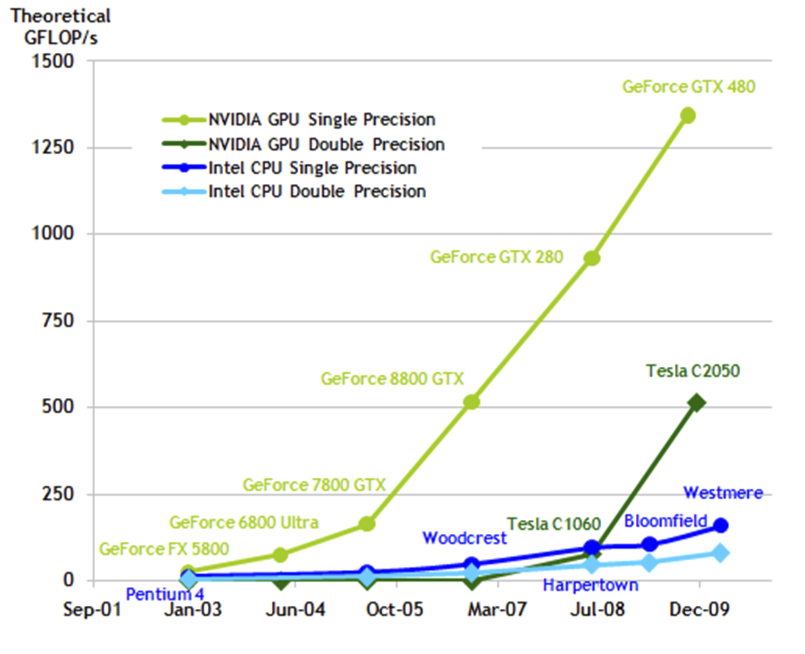
\includegraphics[width=0.7\textwidth]{evolucion-gpu.png}
	\caption{Comparativa de la evolución de los GFlops de las GPUs frente a las CPUs}\label{fig:GPUvsCPU}
\end{figure}

La principal razón de este interés por éste tipo de tecnología se ha visto motivado, principalmente, por tecnologías como CUDA u OpenCl que nos permiten aprovechar las capacidades de las actuales tarjetas gráficas para realizar cálculos y operaciones muy costosas en tiempo de CPU de forma más rápida. Además, permiten un alto grado de paralelismo, lo que puede resultar beneficioso para el desarrollo de ciertos tipos de evaluaciones.

\section{Objetivos}
El presente proyecto final de carrera nace con el objetivo de aprovechar las nuevas arquitecturas gráficas en el entorno de la auditoría de seguridad informática. Igualmente se ha pretendido utilizar un modelo distribuido para mejorar la escalabilidad del sistema y así disponer de una herramienta potente que pueda ser ampliada según la necesidad del momento.

\section{Estructura del documento}

